\chapter{Introduction and Background Research}

\setlength{\parindent}{1em}
\setlength{\parskip}{0em}
\justifying

% You can cite chapters by using '\ref{chapter1}', where the label must
% match that given in the 'label' command, as on the next line.
\label{chapter1}

% Sections and sub-sections can be declared using \section and \subsection.
% There is also a \subsubsection, but consider carefully if you really need
% so many layers of section structure.
\section{Introduction}

Rendering is the process of generating images, or \textit{frames}, of a virtual world (known as a \textit{scene} in rendering). Real-time rendering requires that the generation of these frames is done at a fast enough rate so that the viewer feels they are taking part in an immersive, dynamic experience. Typically, this rate needs to be at least 30 FPS (Frames Per Second), with 60 FPS and beyond being desirable \cite{EffectsOfFrameRate}. This imposes a maximum time budget of 33 to 16 milliseconds in which each frame must be generated, the \textit{frame time}. Real-time rendering presents a compelling problem: how can the visual fidelity of a rendered scene be maximised, whilst adhering to this strict computational budget.

Rendering can be performed using one of two techniques, ray tracing or rasterization. Ray tracing is based on a model that is analogous to how humans perceive light and colour in the real-world. In the real-world, rays of light are produced from many sources, bounce from one object to the next, and eventually reach the viewers eyes. Ray tracing models this same process, but in reverse, with the rays originating from the views eyes, and being traced back to their sources. Provided enough rays are sampled, this approach produces very realistic images. Although ray tracing is the standard in the realm of movie production, its expensive computational requirements lead to frame times in the region of minutes instead of milliseconds~\cite{PixarCars}. Aside from so notable exceptions\footnote{With the advent of hardware accelerated ray tracing on consumer GPUs~\cite{NvidiaTuringArchitecture}, the use of ray tracing to render specific visual phenomena, such as reflections, has seen use in some modern games~\cite{Battlefield5RayTracing}.}, this prohibits its use in real-time applications. As a result, real-time rendering employs another technique, rasterization.

With rasterization, each object in the world is composed of an arrangement of primitive shapes, most commonly, triangles, and their material is described through a number of parameters. When rendering, the world is transformed and projected onto a 2D plane. Within this plane, a fixed region maps to the space of the output image; all triangles that lie outside this region are clipped. The remaining triangles are then split into granular pieces, called \textit{fragments}. A colour is calculated for each fragment by evaluating the amount of light that shines on that fragment in the world, and then how that light interacts with the material of the object that fragment belongs to. Performing this calculation is called \textit{shading}, and how it is done is defined by a \textit{shading model}. After resolving which fragments lie on top of which others, the final image is presented to the user. This whole rasterization process is referred to as the graphics rendering pipeline, and dedicated hardware has been developed to carry it out, the \textit{Graphics Processing Unit} (GPU).

The appearance of the final rendered frames is largely determined by the shading model, and therefore the choice of such a model is crucial. For a long time, the standard shading model used for photo-realistic real-time rendering was Blinn-Phong; it was utilised in popular game engines, and was the default model used in OpenGL's fixed function pipeline~\cite{UnityBlinnPhong}~\cite{UnrealBlinnPhong}~\cite{OpenGLBlinnPhongFixedFunction}. Blinn-Phong is an empirical model: it is based on human observations of how light interacts with materials, rather than the underlying real-world physical rules that govern those interactions~\cite{PhongShading}. Blinn-Phong can produce reasonably realistic images, and is computationally inexpensive - a very desirable trait for real-time rendering. However, due to its non-physically based nature, Blinn-Phong has many issues. Paramount amongst which is its inability to render certain physical phenomena, which limits the realism of rendered frames. Furthermore, the parameters of Blinn-Phong that are used to specify material properties, bear little relation to the characteristics of physical materials. This problem manifests itself in a tight coupling between material parameters and lighting conditions. In order to accurately depict the same physical material under different lighting conditions, it may be necessary to specify differing values for these parameters. This reduces the reusability of assets, making artist workflow more difficult.

In an effort to alleviate these issues, the replacement of Blinn-Phong in favour of physically based shading models has seen widespread adoption. Such models work by evaluating equations that simulate the real world physical interaction of light and objects. Using these models for shading is known as \textit{Physically Based Shading} (PBS), and their use in the wider rendering pipeline is called \textit{Physically Based Rendering} (PBR). PBS represented a seismic shift in the real-time rendering industry, with major game engines migrating to a PBR pipeline~\cite{RealShadingInUnreal}~\cite{MovingFrostbitetoPBR}.

The aim of this project is to investigate the use of physically based shading models in real time rendering. Specifically, I will seek to highlight the benefits of PBS when compared to the technology is superseded, Blinn-Phong shading.

The advantages of using PBS over Blinn-Phong shading can be broadly categorised into two groups: the improvements to artist workflow; and the improved photorealism. As mentioned previously, because of how materials are defined in Blinn-Phong shading they are often not portable between different lighting environments. In contrast, the parameters that determine materials in PBS are based on physical properties. This permits the reuse of materials and assets over different lighting configurations~\cite{MovingFrostbitetoPBR}~\cite{SIGGRAPH2020Course}. Burley outlines how this reduction in the need for "material 're-do's" yields an extremely significant improvement to artist workflow~\cite{Burley2012Physically}. Although these benefits are an important motivating factor for using PBS, the practical issues that arise from trying to investigate and quantify them (I don’t have access to a team of artists) mean that this report will focus solely on exploring those advantages in the latter category – how does PBS render frames that are more photorealistic than Blinn-Phong Shading?

Answering this question by simply commenting on the general perceived realism of a frame when compared to another is a largely subjective exercise. Instead, in a concerted effort to be as objective as possible, I will examine the benefits of PBS by identifying physical phenomena that are more accurately modelled in frames rendered using PBS, than in frames rendered using Blinn-Phong shading. To this end, I will be developing a renderer that can render scenes using both Blinn-Phong shading, and PBS.

% Must provide evidence of a literature review. Use sections
% and subsections as they make sense for your project.
\section{Background Research}

After conducting considerable research within the area of real-time shading models, it is evident that a comparison of the nature described above, has not been done before. Therefore, no descriptions of previous comparisons can be given. Instead, the research presented below thoroughly explores the relevant literature and theory behind Blinn-Phong shading and PBS. This serves two purposes. First, it forms the knowledge that is necessary to carry out the implementation of the renderer. Secondly, it allows the later comparison between the two shading approaches to be performed, and crucially, the results of that comparison to be interpreted and justified.

The research begins with a discussion of the Blinn-Phong shading model. We then delve into the physics of how light interacts with matter, and how this pertains to shading. An exploration of the common constructs used in physically based shading models follows, and then we present several such models. After, we consider how lights can be represented in a physical manner. Finally, we finish by focusing on the wider PBR aspect with a discussion on the nature of shaded pixel values, and the transformations that need to be applied before passing those values to the display. The mathematical notation used throughout this report is outlined in Appendix \ref{MathematicalNotation}.

\subsection{Blinn-Phong Shading} \label{BlinnPhongShading}

\subsubsection{Phong Model}

In 1975, Phong introduced a simple shading model for rendering realistic images~\cite{PhongShading}. The original model is parametrised as the sum of two terms, \textit{diffuse} and \textit{specular}, but in practice it is commonly supplemented with a third term, \textit{ambient}. Each one describes the contribution of a different lighting component. Splitting shading into the evaluation of a diffuse and specular term is common practice, and the physical basis for doing this is explained in section \ref{PhysicsOfLightMatterInteraction}.

An ideal diffuse surface is one that has a Lambertian response to incident light, where the light is reflected in all directions equally~\cite{Lambert}. Therefore, the determining factor in the appearance of such surfaces is the intensity of the incident light, which is a function of the direction of incident light and the orientation of the shaded surface. This is called \textit{Lambert's Cosine Law}~\cite{Lambert}. The diffuse term encodes the lighting effects of parity between a primitive's surface orientation and the direction of the light, with surfaces facing the light being illuminated more intensely than those facing away from it. This behaviour is formulated as:

\begin{equation}
	\vect{c}_{shaded_{diff}} = \vect{c}_{surface_{diff}}\vect{c}_{light_{diff}}(\vect{n}\cdot\vect{l})^+
\end{equation}

\begin{math}\vect{c}_{shaded_{diff}}\end{math}, \begin{math}\vect{c}_{surface_{diff}}\end{math}, and \begin{math}\vect{c}_{light_{diff}}\end{math} are the RGB triplets that represent the diffuse colour of the shaded fragment, the diffuse colour of the surface, and the diffuse colour of the incident light respectively. This separation of the light and surface colours into separate components was not present in Phong's original model. However, many implementations have increased the flexibility of the model by exposing these additional parameters~\cite{LightingModelForComputerAnimators}. The \textit{normal}, \begin{math}\vect{n}\end{math}, is the unit vector pointing away from the surface at the shaded point, giving the orientation of the surface.  The \textit{light direction}, \begin{math}\vect{v}\end{math}, is the unit vector pointing in the direction of the incident light. See Figure \ref{fig:PrincipleVectors} for an illustration of the principle vectors used in the Phong shading model (and indeed, by most shading models). The dot product of two unit vectors is equivalent to taking the cosine of the angle between them. Therefore, \begin{math}(\vect{n}\cdot\vect{l})^+\end{math} will increase from 0 to 1 as the angle between the incident light direction and the surface normal decreases. Thus, the more aligned the surface orientation and light direction are, the greater the intensity of the diffuse term. Negative values of the dot product indicate that the light direction is underneath the surface. In these cases the light is not incident upon the surface at all, so the dot product is clamped to 0.

The specular term of the model captures the ability for surfaces to exhibit highlights due to surface reflections. When light is incident upon a surface, it will experience some reflection, and when the reflected light is aligned with the direction of the viewer, this is perceived as a region of increased illumination, a \textit{specular highlight}. The formula for the specular term is:

\begin{equation}
	\vect{c}_{shaded_{spec}} = \vect{c}_{surface_{spec}}\vect{c}_{light_{spec}}((\vect{r}\cdot\vect{v})^+)^{surface_{shininess}}
\end{equation}

Where \begin{math}\vect{r}\end{math} is the reflection of the incident light about the surface normal, and is defined as:

\begin{equation}
	\vect{r} = 2(\vect{n}\cdot\vect{l})\vect{n} - \vect{l}
\end{equation}

The RGB triplets are similar to those in the diffuse equation, except these are specific to the specular response. Phong's original model had the colour of the specular highlight be the same as the overall colour of the light (not split into separate diffuse and specular components). This gave all materials an overly plastic appearance. Introducing the \begin{math}\vect{c}_{surface_{spec}}\end{math} and \begin{math}\vect{c}_{light_{spec}}\end{math} variables allows for the colour of the specular highlight to be fully configurable, mitigating this issue~\cite{LightingModelForComputerAnimators}. The \textit{view vector}, \begin{math}\vect{v}\end{math}, is the unit vector pointing in the direction of the viewer. The dot product measures the alignment between the view direction, and the direction of the reflected incident light. The \begin{math}surface_{shininess}\end{math} parameter determines the concentration of the reflected light rays. The higher the value, the more focused the reflected rays are, the smaller the specular highlight becomes, and the shinier the object appears. Typical values range from 1 to 100.

Finally, we have the ambient term. In the model developed so far, if a shaded point is not directly visible from a light source, then it will be black. In reality, such points are never completely unilluminated - rays from light sources will bounce around the environment, eventually lighting these obscured areas. So far we have only considered \textit{direct illumination}; the ambient term is used to crudely approximate the lighting that is a consequence of this \textit{indirect illumination}:

\begin{equation} \label{eq:BlinnPhongAmbient}
	\vect{c}_{shaded_{ambi}} = \vect{c}_{surface_{ambi}}x
\end{equation}

\begin{math}\vect{c}_{surface_{ambi}}\end{math} controls the colour of the ambient shading. Typically, it is just set equal to \begin{math}\vect{c}_{surface_{diff}}\end{math}. \begin{math}x\end{math} is a constant value defined for the whole scene, rather than per light, and controls the amount of indirect illumination that occurs. Small values of \begin{math}x\end{math} should be used, as anything too large will make the scene look unrealistically bright - lighting via indirect illumination is usually quite subtle as light loses energy every time it reflects of a surface.

These three terms are summed together to give the overall Phong shading model:

\begin{equation}
	\vect{c}_{shaded} = \vect{c}_{shaded_{ambi}} + \vect{c}_{shaded_{diff}} + \vect{c}_{shaded_{spec}}
\end{equation}

\begin{figure}[h]
	\centering
	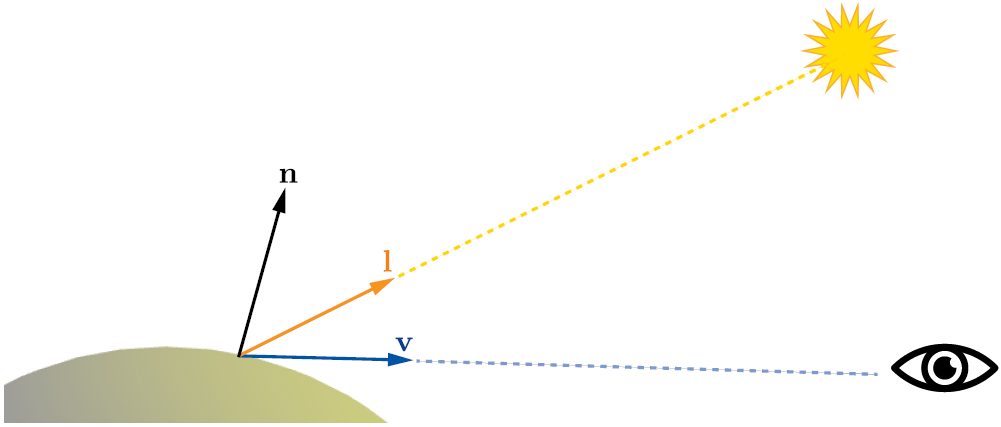
\includegraphics[width=8cm]{PrincipleVectors}
	\caption{The surface normal \begin{math}\vect{n}\end{math}, light direction \begin{math}\vect{l}\end{math}, and view vector \begin{math}\vect{v}\end{math}. Taken from~\cite{RTR4}}
	\label{fig:PrincipleVectors}
\end{figure}

\subsubsection{Blinn-Phong Model}

One of the issues with the Phong shading model is made apparent when viewing a rough (low \begin{math}shininess\end{math} value) surface from a direction close to the incident light. The corresponding reflected light vector makes an angle with the view direction that is greater than 90$^{\circ}$. In this instance, the dot product \begin{math}\vect{r}\cdot\vect{v}\end{math} evaluates to a negative value, and is thus clamped to 0, leading to no specular contribution. However, for very rough surfaces, the specular highlight is so wide that even at these greater angles, there should still be a specular contribution. See Figure \ref{fig:PhongIssue} for an illustration of the problem.

In 1977, Blinn remedied this issue by modifying the Phong shading model with a more accurate specular term~\cite{BlinnModelsOfLightReflection}. He utilised the half vector, \begin{math}\vect{h}\end{math}, dispensing with the reflected light vector, \begin{math}\vect{r}\end{math}, and replaced the existing specular dot product with \begin{math}\vect{h}\cdot\vect{n}\end{math}. \begin{math}\vect{h}\end{math} is a unit vector pointing in the direction that is halfway between the \begin{math}\vect{l}\end{math} and \begin{math}\vect{v}\end{math} vectors. It is calculated as:

\begin{equation}
	\vect{h} = \frac{\vect{l} + \vect{v}}{\norm{\vect{l} + \vect{v}}}
\end{equation}

Blinn's specular term emulates the overall behaviour of the original Phong term. As the (now conceptual) reflection vector \begin{math}\vect{r}\end{math} aligns with \begin{math}\vect{v}\end{math}, so does the half vector \begin{math}\vect{h}\end{math} align with the surface normal \begin{math}\vect{n}\end{math}. Crucially though, \begin{math}\vect{h}\cdot\vect{n}\end{math} will only evaluate to a negative value, and subsequently be clamped to 0, if \begin{math}\vect{l}\end{math} or \begin{math}\vect{v}\end{math} is beneath the surface. Therefore, the scenario in which rough surfaces were being shaded incorrectly with no specular contribution, is resolved. See \ref{fig:BlinnFix} for an illustration.

\begin{figure}[h]
	\begin{subfigure}{0.48\textwidth}
		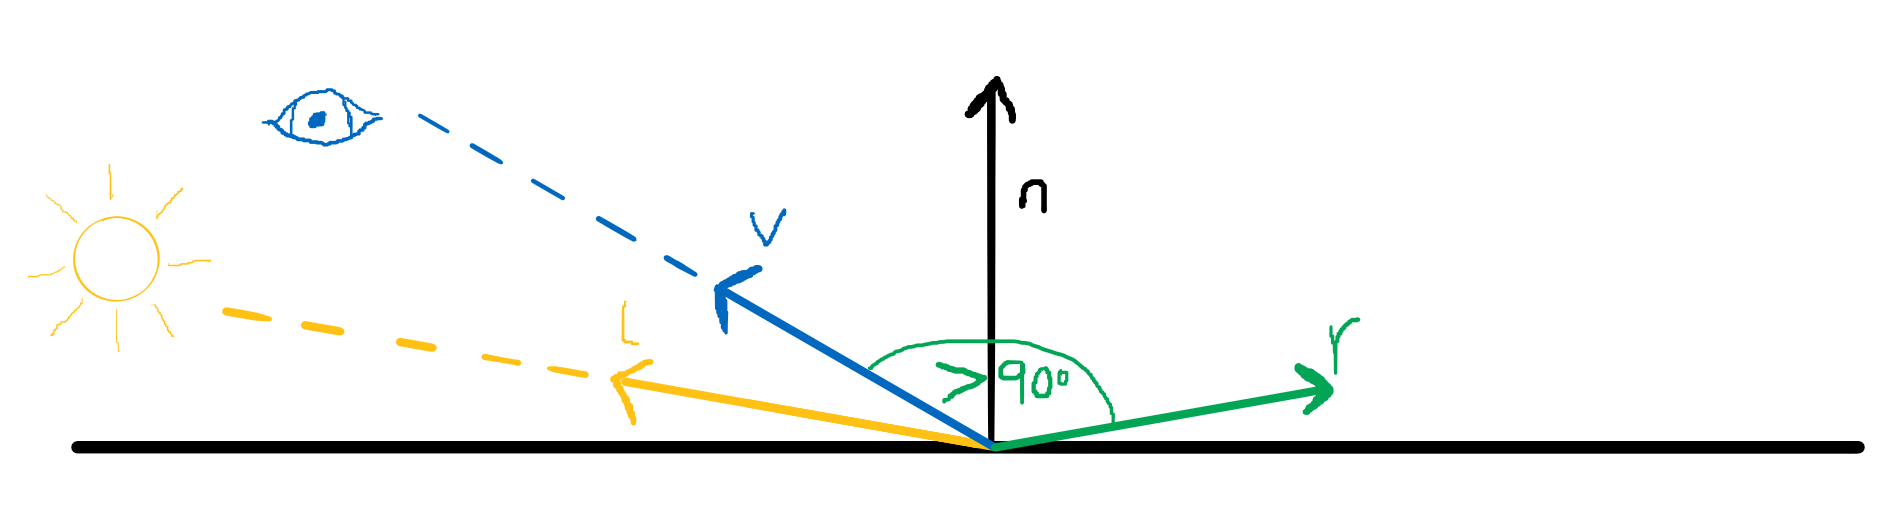
\includegraphics[width=\linewidth]{PhongIssue}
		\caption{The angle between \begin{math}\vect{r}\end{math} and \begin{math}\vect{v}\end{math} can exceed 90$^{\circ}$ whilst \begin{math}\vect{l}\end{math} and \begin{math}\vect{v}\end{math} are still above the surface}
		\label{fig:PhongIssue}
	\end{subfigure}
	\hspace*{\fill}
	\begin{subfigure}{0.48\textwidth}
		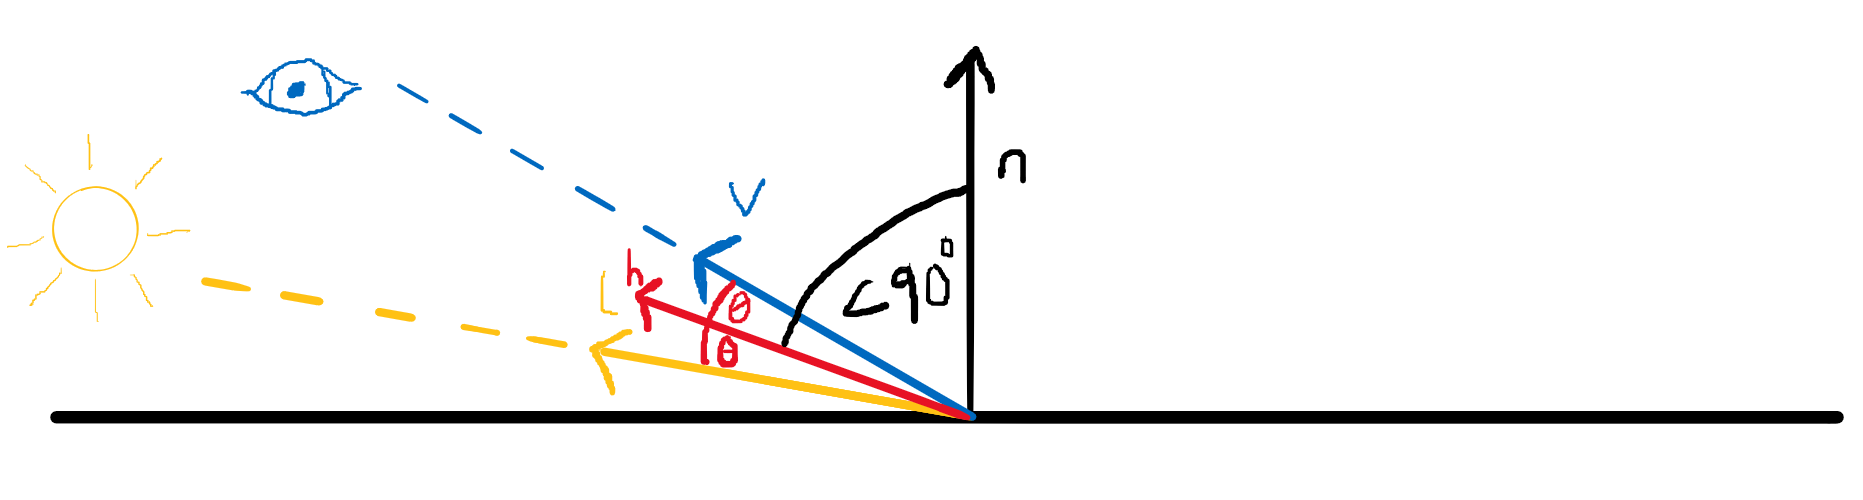
\includegraphics[width=\linewidth]{BlinnFix}
		\caption{The angle between \begin{math}\vect{h}\end{math} and \begin{math}\vect{n}\end{math} can't exceed 90$^{\circ}$ without \begin{math}\vect{l}\end{math} or \begin{math}\vect{v}\end{math} being below the surface }
		\label{fig:BlinnFix}
	\end{subfigure}
	\caption{}
\end{figure}

Blinn's modification to the Phong model is known as the Blinn-Phong shading model, and it produces more realistic images than the original. The model is formulated as:

\begin{equation} \label{eq:BlinnPhong}
	\vect{c}_{shaded} = p_{ambi} + p_{diff}(\vect{n}\cdot\vect{l})^+ + p_{spec}((\vect{h}\cdot\vect{n})^+)^{surface_{shininess}}
\end{equation}

where

\begin{center}
	\begin{math}p_{ambi} = \vect{c}_{surface_{ambi}}x\end{math} \\
	\begin{math}p_{diff} = \vect{c}_{surface_{diff}}\vect{c}_{light_{diff}}\end{math} \\
	\begin{math}p_{spec} = \vect{c}_{surface_{spec}}\vect{c}_{light_{spec}}\end{math}
\end{center}

Expressing the model in this way draws attention to the relative proportions of each component that contributes to the overall shading. These proportions, \begin{math}p\end{math}, are modulated via lighting parameters:  \begin{math}light\end{math} variables and \begin{math}x\end{math}; and material parameters: \begin{math}surface\end{math} variables.

In scenes with multiple lights, the diffuse and specular terms of equation \ref{eq:BlinnPhong} are evaluated for each one. Then these intermediate values are summed together with the scene's ambient term to get the overall colour of the fragment.

\subsection{Physics of Light-Matter Interaction} \label{PhysicsOfLightMatterInteraction}

\subsubsection{Visible Light}

The Electromagnetic spectrum is a distribution of wavelengths, of which a small section is spanned by visible light. More specifically, visible light are those electromagnetic (EM) waves with a wavelength between 400nm, violet, and 700nm, red. Typically, visible light will contain a combination of wavelengths within this range. We can express light waves as a relation between each wavelength and its associated energy, in what are known as Spectral Power Distributions (SPD). Although s exist that store light as SPDs, the negative performance implications that accompany this approach mean that in practice, an abstraction is often used~\cite{SpectralRendering}. This abstraction exploits the relative imprecision of the human visual perception system. Using a linear combination of three wavelengths, R, G and B, we can accurately represent any visible light wave and colour~\cite{RGBColours}. Renderers store this combination as an RGB triplet, with each value giving the weight of its associated wavelength.

The area of study concerned with quantifying EM waves is called \textit{Radiometry}~\cite{IntroToRadiometry}. Several \textit{radiometric} measurements exist, with the most commonly used one in rendering being \textit{radiance}, \begin{math}L\end{math}. Radiance measures the power of a single EM ray. It's defined as energy over time (power), with respect to area and direction: \begin{math}W/m^2sr\end{math}. Power is expressed in Watts, area in metres squared, and direction in \textit{Steradians}. Steradians are to solid angles, what radians are to normal angles. A solid angle is the 3D version of a normal 2D angle. Evaluating a shading model is equivalent to computing the radiance of a single light ray that goes from the shaded fragment to the viewer. See section \ref{PrinciplesOfShading} for more details.

\subsubsection{Light Interaction with Matter}

The way in which light interacts with matter is characterised by the matter's \textit{index of refraction} (IOR). The IOR defines the speed that light travels through the matter, given in relative terms to the speed of light in a vacuum~\cite{HowLightInteractsWithMatter}. The IOR can also be extended to describe the absorption qualities of the matter, in what is known as the \textit{complex index of refraction}. Some matter absorbs light waves by converting part of their energy to heat, causing an attenuation of the lights amplitude and intensity. Both forms of refractive index can vary by wavelength.

Light interacts with matter in three ways~\cite{HoffmanPBSBackground}. When light is travelling through a volume of matter with a uniform IOR, a \textit{homogenous medium}, it will not deviate in its direction. However, the absorption value of the IOR may cause the light to undergo changes in intensity, and if this varies by wavelength, changes in colour also. Water is an example of a homogenous medium that absorbs light, but mostly around the red wavelengths - this gives its intrinsic blue and green colour~\cite{HowLightInteractsWithMatter}.

Light behaves differently in a \textit{heterogeneous medium}, where the IOR is not uniform. If light encounters a change in IOR that takes place over a distance smaller that a light wavelength, it will \textit{scatter} into multiple directions. The amount of scattering varies by wavelength. The frequency of scattered light will be the same as the original light. The only exception to this is when fluorescence or phosphorescence phenomena is present, but since this is very rare in the real world, we ignore such scenarios when rendering. In the likely case that the original light is comprised of a distribution of different wavelengths and frequencies, each one will interact independently. If interacting with a single isolated particle, the scattered light will move in all directions, but at different intensities~\cite{RTR4}.

Finally, light can interact with matter in a manner that is opposite to that of absorption. \textit{Emission} can take place within matter, where other forms of energy are converted to light energy, and light is emitted. Light sources work in this way.

In general, the appearance of most media is as a consequence of both scattering and absorption.

\subsubsection{Light Incident to Surfaces}

When shading, we are interested in simulating what happens when light is incident upon the surface of an object. When this interaction occurs, two properties effect the outcome: the geometry of the surface, and the nature of the substances either side of the surface~\cite{RTR4}~\cite{DiffuseSpecularAtSurfaces}.

We first consider the substance factor and assume that the surface's geometry is a perfectly flat plane. An object's surface can then be described as a flat two-dimensional boundary separating two volumes with differing IORs. In rendering it is typical that the outer volume is comprised of air, which has an IOR of 1 (or to be exact, 1.0003). The inner volume has an IOR defined by the material of the object. Any light wave that impinges on the boundary will encounter an abrupt change in the IOR, which - as explained above - will result in scattering. Because the boundary is a flat plane, the nature of this scattering is well defined: some of the scattered waves will continue moving into the surface, the \textit{transmitted wave}, and the others will be reflected at the surface and move away, the \textit{reflected wave}. The reflected wave propagates in a direction that is the reflection of the incident wave about the surface normal. The transmitted wave will undergo \textit{refraction} and move at an angle of \begin{math}\theta_t\end{math}, which is defined by the relative IOR of the two volumes and the angle of the incident light, \begin{math}\theta_i\end{math}~\cite{SnellsLaw}. See Figure \ref{fig:BoundaryScattering} for an illustration of this scattering behaviour. The proportion of reflected versus transmitted light follows the Fresnel equations, which are explained in section \ref{FresnelReflectance}~\cite{PractitionersReflectionModels}. The transmitted wave will interact with the interior of the object in the same way as light interacts with any medium - it will experience some degree of scattering and absorption.

\begin{figure}[h]
	\centering
	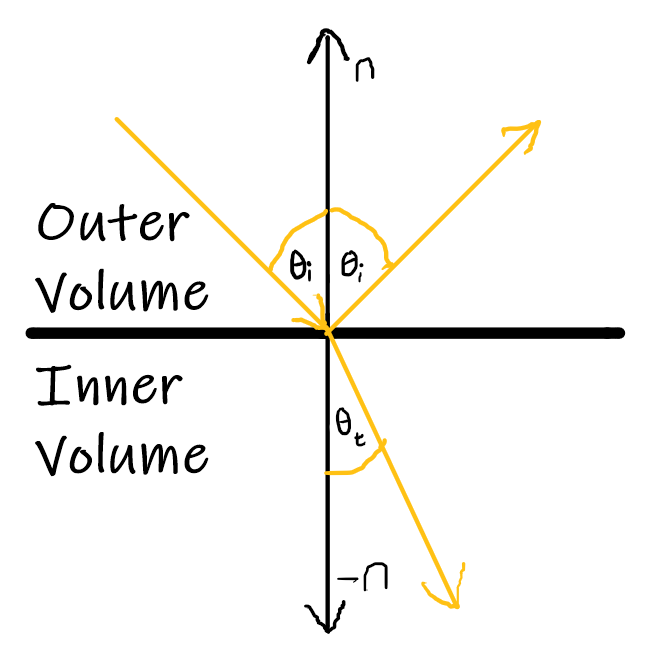
\includegraphics[width=5cm]{BoundaryScattering}
	\caption{The scattering that occurs when light is incident upon a perfectly flat boundary}
	\label{fig:BoundaryScattering}
\end{figure}

Now we focus on the effect that geometry plays when light is incident on a surface. The case we have just seen of a perfectly flat surface is of course not possible; all surfaces have some variation in their geometry. Any irregularities in the geometry that are smaller than a single light wavelength do not have any impact. Irregularities larger than 100 wavelengths constitute their own local plane of flatness, with their own orientation. Irregularities that have a size within this range cause the surface-light interaction to behave differently to that described above, with phenomena such as \textit{diffraction} also being present. However, when shading we typically stay within the realm of \textit{geometrical optics}, which means we ignore the effects of these irregularities\footnote{Although not widely used in real-time rendering, some shading models do exist for simulating the phenomena that occur when light interacts with geometrical irregularities of this size~\cite{ReflectionAndDiffractionModel}}~\cite{DiffuseSpecularAtSurfaces}. Geometrical optics strictly deals with light as rays, not waves, and these rays always intersect locally flat planes with behaviour described above and illustrated in Figure \ref{fig:BoundaryScattering}. When shading, a single pixel or fragment will span much more than 100 wavelengths, so we need to account for the local planes of flatness that exist in this region. Irregularities at this scale are referred to as \textit{microgeometry}. As a consequence of microgeometry, each point on the surface will reflect light in one direction, and refract it in another. Therefore, when determining the effect of microgeometry over a whole pixel, we can consider the light to be reflected and refracted in many directions. These directions are defined by the individual orientations of the points, and quantified by regarding them as a distribution of normals. The tighter the distribution, the tighter the spread of reflected and refracted directions. The roughness of the material directly controls the variance of this distribution. Section \ref{MicrofacetTheory} discusses this in detail.

\subsubsection{Transmitted Light Interaction}

As explained previously, the light that is transmitted into the interior of an object will experience a mixture of scattering and absorption. In some materials, the light will be scattered enough that it is re-emitted at the surface of the object in a process called \textit{subsurface scattering}~\cite{Spectroscopy}. See Figure \ref{fig:SubsurfaceScattering} for an illustration. The distance between the subsurface scattered light and the original incident light is determined by the nature of the material, and is very important when shading. If the subsurface scattering distances are smaller than the span of one pixel, as is common for most materials, we call it \textit{local subsurface scattering}~\cite{PractitionersReflectionModels}. In such cases, the subsurface scattered light is combined with the light reflected from the object surface to form a local shading model, where the outgoing light at one point is wholly dependent on the incoming light at that same point. Subsurface scattered light will encounter protracted interactions of absorption and scattering in the interior of the object, before finally being re-emitted. Therefore, it will have a distinctly different colour to the surface reflected light~\cite{ReflectionFromLayeredSurfaces}. For this reason, shading is split into two different terms: the \textit{specular term} captures the light reflected at the object surface, whilst the \textit{diffuse term} models the local subsurface scattering. See Figure \ref{fig:SpecularAndDiffuse} for an illustration of these two shading components.

Shading is more complex when the subsurface scattering distances are larger than a single pixel. \textit{Global subsurface scattering} is often encountered when rendering skin or wax, and although special models have been developed to shade these materials, it is beyond the scope of this report~\cite{SeparableSubsurfaceScattering}.

\begin{figure}[h]
	\begin{subfigure}{0.48\textwidth}
		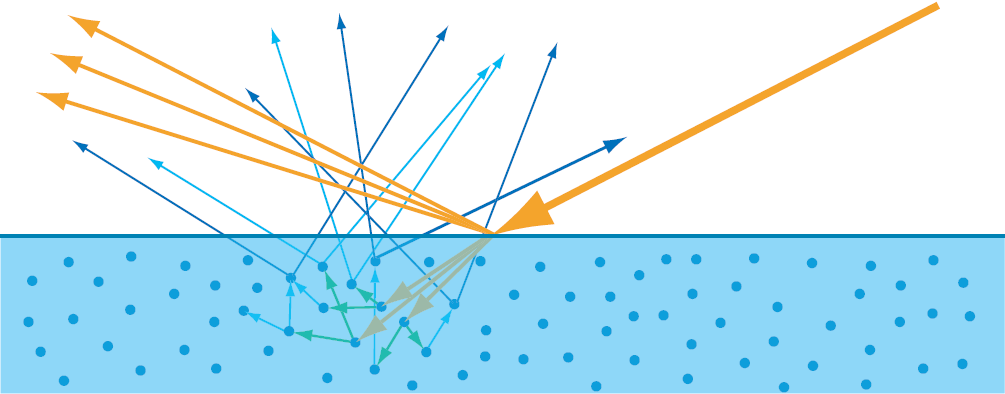
\includegraphics[width=\linewidth]{SubsurfaceScattering}
		\caption{Light is re-emitted at the surface of an object by means of subsurface scattering}
		\label{fig:SubsurfaceScattering}
	\end{subfigure}
	\hspace*{\fill}
	\begin{subfigure}{0.48\textwidth}
		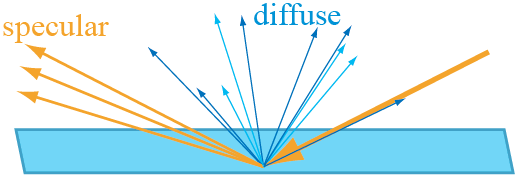
\includegraphics[width=\linewidth]{SpecularAndDiffuse}
		\caption{When shading a point we consider the specular and diffuse terms}
		\label{fig:SpecularAndDiffuse}
	\end{subfigure}
	\caption{Taken from~\cite{RTR4}}
\end{figure}

\subsubsection{Metals and Dielectrics}

The proportion of scattering and absorption that transmitted light induces varies by material. There are two main categories of materials that we encounter day-to-day: metals and \textit{dielectrics}. Metals immediately absorb any transmitted light, meaning their appearance is solely provided by the specular term. Most other materials are non-conductive, called dielectrics. These materials do allow for subsurface scattering, so both the specular and diffuse terms characterise their appearance.

\subsection{Principles of Shading} \label{PrinciplesOfShading}

\subsubsection{The Reflectance Equation}

When rendering, we model the viewer as a camera placed at point \begin{math}\vect{c}\end{math}. The camera projects a 2D matrix of photosensitive sensors that map to pixels on the display. By combining outputs of all the sensors, we get the final rendered image. For each of the sensors, we have a ray that originates from \begin{math}\vect{c}\end{math}, intersects the sensor, and then continues into the scene; this ray propagates in the opposite direction to the view vector, \begin{math}\vect{-v}\end{math}. With PBS, we obtain the colour of a sensor by calculating the incoming radiance to \begin{math}\vect{c}\end{math} in the direction \begin{math}\vect{-v}\end{math}. Thus, the final rendered image is given by calculating incoming radiance to \begin{math}\vect{c}\end{math} over the set of all \begin{math}\vect{-v}\end{math} vectors.

A scene is comprised of a number of objects separated by media. Typically when rendering, we just consider all media to be air. Air is a medium that exhibits very little scattering nor absorption, so its effect on radiance is minimal and can be ignored. Therefore, incoming radiance to \begin{math}\vect{c}\end{math} in the direction \begin{math}\vect{-v}\end{math}, is equivalent to outgoing radiance from point \begin{math}\vect{p}\end{math} along \begin{math}\vect{v}\end{math}, where \begin{math}\vect{p}\end{math} is the intersection point that the closest object will make with a ray that travels along \begin{math}\vect{-v}\end{math}. This quantity is defined as \begin{math}L_o(\vect{p}, \vect{v})\end{math} and is calculated by means of the \textit{reflectance equation}:

\begin{equation}
	L_o(\vect{p}, \vect{v}) = \int_{\vect{l}\in\Omega}f(\vect{l}, \vect{v})L_i(\vect{p}, \vect{l})(\vect{n}\cdot\vect{l})\,d\vect{l}
\end{equation}

The \begin{math}\vect{l}\in\Omega\end{math} in the integral subscript says that the integral should be performed over all directions \begin{math}\vect{l}\end{math} that exist in the unit hemisphere \begin{math}\Omega\end{math}, which is centred on \begin{math}\vect{p}\end{math} and orientated along the surface normal \begin{math}\vect{n}\end{math}. In this way, the incoming radiance from all possible light sources is considered. The product within the integral gives the outgoing radiance from \begin{math}\vect{p}\end{math} along \begin{math}\vect{v}\end{math} for a singular incident light direction \begin{math}\vect{l}\end{math}. The effect of the integration is to sum over all the individual components of outgoing radiance, to obtain the total value. This formulation is consistent with the shading scenario that was introduced in the "Transmitted Light Interaction" section of \ref{PhysicsOfLightMatterInteraction}, except it is expressed from a slightly different perspective: instead of keeping the incoming light direction constant and considering many outgoing light directions, we are now keeping the outgoing light direction constant, and considering all possible incoming light directions. Note that this is indeed a local shading model, with all outgoing light at \begin{math}\vect{p}\end{math} being wholly dependent on incoming light at \begin{math}\vect{p}\end{math}. A physically based shading model computes the reflectance equation using physically based implementations of \begin{math}f\end{math} and \begin{math}L_i\end{math}. We now discuss each of the factors of the integral's product in turn.

\subsubsection{The BRDF}

The \textit{bidirectional reflectance distribution function} (BRDF), \begin{math}f(\vect{l}, \vect{v})\end{math}, was first introduced by Nicodemus et al in 1977 \cite{OriginalBRDF}. For a given \begin{math}\vect{l}\end{math} and \begin{math}\vect{v}\end{math}, the BRDF gives the ratio of incident light in direction \begin{math}\vect{l}\end{math}, which after striking the surface, is reflected in direction \begin{math}\vect{v}\end{math}. The function is a distribution over all possible values of \begin{math}\vect{l}\end{math} and \begin{math}\vect{v}\end{math} that lie in the unit hemisphere introduced above, and thereby it completely describes a surface's local reflectance response to incident light. Local reflectance encompasses both surface reflection and local subsurface scattering. Variations of the BRDF exist which seek to capture other light-matter interactions, such as the BSSRDF which accounts for the influence of global subsurface scattering~\cite{PracticalModelForSubsurfaceLightTransport}.

As explained previously, scattering and absorption - the two phenomena that underpin local reflectance - vary by wavelength. Therefore, the BRDF also needs to vary by wavelength, so the ratios it returns are given as RGB triplets.

For a BRDF to be considered physically plausible, two constraints must hold. The first is called the Helmholtz reciprocity and states that \begin{math}f(\vect{l}, \vect{v}) = f(\vect{v}, \vect{l})\end{math}~\cite{HelmholtzReciprocity}. BRDFs used in rendering don't often comply with this equality, but still look physically correct~\cite{RTR4}. The second constraint is imposed by conservation of energy: the outgoing light energy cannot exceed the incoming light energy. In real-time rendering, exact adherence to this principle is not required, but respecting it in the approximate sense is very important - otherwise, objects will be rendered as overly bright and unrealistic~\cite{RTR4}\cite{MovingFrostbitetoPBR}.

Constructing a BRDF can be accomplished in two ways: via optical measurements of real materials, or by leveraging mathematical formulas. Ward discusses the use of a \textit{Gonioreflectometer} to measure BRDFs of real world materials \cite{MeasuringAnisotropicReflections}. This process is time consuming and thus it's use in rendering is impractical. Instead, we construct BRDFs using parametrised mathematical formulas. The parameters involved are properties of the object's material. If the material properties are specified over every point on the object - which is commonly practiced in graphics by utilising textures - then this is equivalent to defining a BRDF for every point on the object's surface. As mentioned, the local reflectance response of a surface is split into specular and diffuse terms when shading. Naturally, this extends to the BRDF itself, and it is expressed as the sum of a specular BRDF and a diffuse BRDF.

These parametrised mathematical formulas can be categorised as either empirical or physically based. Although not represented explicitly, the Blinn-Phong shading model detailed in section \ref{BlinnPhongShading} defines within it an empirical BRDF. Physically based BRDFs lie at the very heart of PBS, and sections \ref{BRDFBuildingBlocks}, \ref{SpecularBRDFs} and \ref{DiffuseBRDFs} are concerned with investigating them.

Figure \ref{fig:ExampleBRDF} gives an example of a BRDF. Visualising a BRDF is difficult as it is a function of four parameters (two angles per vector, one for elevation and another for rotation), so the Figure adopts the common approach of keeping the incident light direction constant.

\begin{figure}[h]
	\centering
	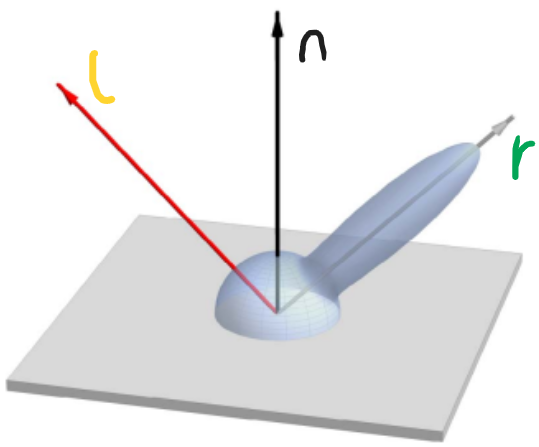
\includegraphics[width=4cm]{ExampleBRDF}
	\caption{An example BRDF. The spherical shape represents the diffuse response, and the lobe represents the specular response. Notice that the specular lobe is concentrated around the reflection vector \begin{math}\vect{r}\end{math}. Adapted from~\cite{FaulInfluenceOfFresnelEffect}.}
	\label{fig:ExampleBRDF}
\end{figure}

\subsubsection{Incoming Radiance}

The incoming radiance term, \begin{math}L_i(\vect{p}, \vect{l})\end{math}, represents the light that originates in direction \begin{math}\vect{l}\end{math} and strikes the surface at point \begin{math}\vect{p}\end{math}. Illumination and light sources are discussed in depth in section \ref{Illumination}.

\subsubsection{Dot Product Term}

The dot product term, \begin{math}(\vect{n}\cdot\vect{l})\end{math}, is the same as that discussed in section \ref{BlinnPhongShading}. It fulfils the same purpose, going from 0 to 1 as the light direction approaches the surface normal. When multiplied by the incoming radiance term, it appropriately scales the amount of illumination. It's also common for this dot product to be clamped to 0, so that contributions from light sources below the surface are ignored.

\subsection{BRDF Building Blocks} \label{BRDFBuildingBlocks}

Most physically based BRDFs are built upon the same set of standard mathematical functions and theory. The individual BRDFs then differ from one another in how these functions are implemented and compiled together. We first detail the standard mathematical building blocks, and then specific specular and diffuse BRDFs are discussed in sections \ref{SpecularBRDFs} and \ref{DiffuseBRDFs} respectively.

\subsubsection{Fresnel Reflectance} \label{FresnelReflectance}

In section \ref{PhysicsOfLightMatterInteraction}, the behaviour of light that impinges upon a surface was said to be dependent on two factors: the substances either side of the surface, and the geometry of the surface. As alluded to, the Fresnel equations describe how light behaves due to the substances. We again assume a perfectly flat boundary separating an outer and inner substance, which have IORs of \begin{math}n_1\end{math} and \begin{math}n_2\end{math} respectively. The Fresnel reflectance, \begin{math}F\end{math}, gives the proportion of incoming light that is reflected at the boundary. Due to the conservation of energy, the amount of transmitted light can then also be easily obtained. \begin{math}F\end{math} varies by wavelength so is expressed as an RGB triplet. Given values of \begin{math}n_1\end{math} and \begin{math}n_2\end{math}, \begin{math}F\end{math} is then a function of incident light angle, \begin{math}F(\theta_i)\end{math}. As mentioned, in rendering it's typical for the outer substance to be air with an IOR of 1, and thus we will be in a scenario of \textit{external reflection}, where \begin{math}n_1 < n_2\end{math}.

In the case of external reflectance, \begin{math}F(\theta_i)\end{math} always follows the same pattern~\cite{RTR4}. When \begin{math}\theta_i = 0^\circ\end{math}, \begin{math}F\end{math} will be equal to the intrinsic specular colour of the inner substance, \begin{math}F_0\end{math}. Between 0$^{\circ}$ and 90$^{\circ}$, \begin{math}F\end{math} will then increase non-linearly towards white; slowly for most of the interval and then rising rapidly when close to 90$^{\circ}$. The tendency for surfaces to exhibit increased reflection at glancing angles is called the \textit{Fresnel effect}.

Using the Fresnel equations themselves is not possible in real-time rendering because \begin{math}n_1\end{math} and \begin{math}n_2\end{math} must be known for all wavelengths of visible light, and this data is not available~\cite{SchlickApproximation}. Instead, approximations that rely on the pattern outlined above are utilised. These are functions that depend in part on \begin{math}F_0\end{math}, which is known for many materials.

\begin{math}F_0\end{math} is defined by the object's material parameters. Dielectrics all have very low \begin{math}F_0\end{math} values, grouping around the \begin{math}(0.04, 0.04, 0.04)\end{math} mark - a fact that is exploited by many physically based shading models. This means dielectrics only reflect a noticeable amount of light at very glancing angles. Metals on the other hand have much higher \begin{math}F_0\end{math} values, with each RGB channel typically exceeding 0.5. Akenine-M\"{o}ller et al give a comprehensive overview of \begin{math}F_0\end{math} values for different materials~\cite{RTR4}.

\subsubsection{Microfacet Theory} \label{MicrofacetTheory}

We now revisit the role that the surface geometry plays in local reflectance. Recall that when rendering, a single pixel will lie over many pieces of microgeometry. The reflectance at the shading point is then determined by the aggregation of the individual interactions that light will have with each piece of microgeometry. We reason about these interactions by utilising \textit{microfacet theory}. The theory states that microgeometry be modelled as a collection of perfectly flat planes called \textit{microfacets}~\cite{BlinnModelsOfLightReflection}. Such a model is effective at representing many real world materials~\cite{ExperimentalAnalysisOfBRDF}. The microfacets' impact on surface reflectance is described by a \textit{Normal Distribution Function} (NDF), a \textit{masking-shadowing function}, and a \textit{micro-BRDF}.

The NDF, \begin{math}D(\vect{m})\end{math}, statistically describes the orientations of the microfacets over the macrosurface (the shaded point when viewed at the pixel scale)~\cite{HeitzMicrofacetTheory}. The more microfacets that have a normal of \begin{math}\vect{m}\end{math}, the higher the value of \begin{math}D(\vect{m})\end{math}. Typically, surfaces posses a distribution of microfacet normals that is concentrated around the normal of the macrosurface \begin{math}\vect{n}\end{math}.

Whilst the NDF describes the orientations of the microfacets, it doesn't describe their arrangement, which also plays a significant role in how light reflects off the macrosurface. Some microfacets will not be visible from the view vector \begin{math}\vect{v}\end{math} because they are occluded by other microfacets. This is known as \textit{masking}. Only those microfacets that are not masked by others will be visible to the viewer and thus contribute to the shading. Furthermore, some microfacets will be occluded so they aren't visible to the incoming light direction \begin{math}\vect{l}\end{math}. This is known as \textit{shadowing}. Microfacet theory only models the first interaction between light and microfacet, thus, only those microfacets that are not shadowed by others are assumed to contribute to the local reflectance~\cite{HeitzMicrofacetTheory}. In reality, incident light will bounce multiple times within a surfaces microgeometry, meaning even microsurfaces that aren't visible directly from the light will exhibit some reflectance. This is known as \textit{interreflection}. Surfaces can look overly dark and conservation of energy will be violated when this phenomena is not modelled~\cite{MultipleScatteringMicrofacet}. Figure \ref{fig:MaskingAndShadowing} illustrates masking and shadowing. The appropriately named \textit{masking-shadowing function}, \begin{math}G(\vect{l}, \vect{v}, \vect{m})\end{math}, accounts for the effects of masking and shadowing. It provides the fraction of microfacets with normal \begin{math}\vect{m}\end{math} that are visible from directions \begin{math}\vect{v}\end{math} and \begin{math}\vect{l}\end{math}~\cite{BlinnModelsOfLightReflection}.

\begin{figure}[h]
	\begin{subfigure}{0.48\textwidth}
		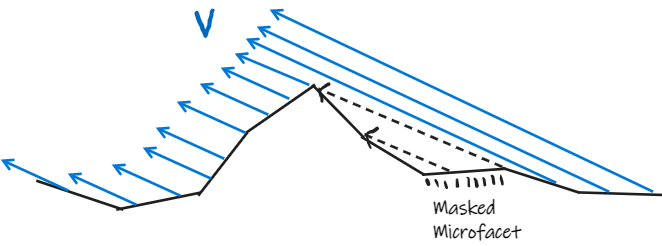
\includegraphics[width=\linewidth]{Masking}
		\caption{Some microfacets are masked by others}
	\end{subfigure}
	\hspace*{\fill}
	\begin{subfigure}{0.48\textwidth}
		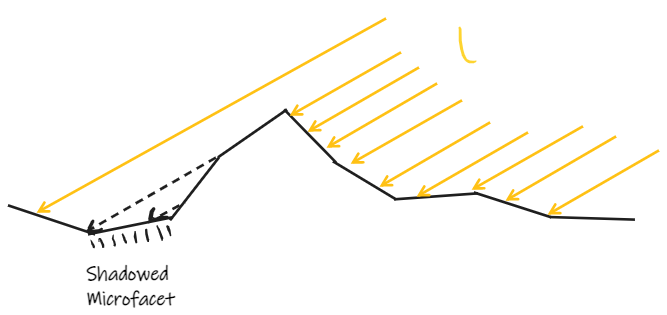
\includegraphics[width=\linewidth]{Shadowing}
		\caption{Some microfacets are shadowed by others}
	\end{subfigure}
	\caption{}
	\label{fig:MaskingAndShadowing}
\end{figure}

The micro-BRDF, \begin{math}f_\mu(\vect{l}, \vect{v}, \vect{m})\end{math}, describes how light is reflected of an individual microfacet. There are two common choices for micro-BRDF. It's typical in a specular (macro) BRDF, that all the microfacets are modelled as perfect mirrors~\cite{CookTorrance}. This means that the micro-BRDF will reflect an incident light ray \begin{math}\vect{l}\end{math} in only one direction: \begin{math}\vect{l}\end{math} reflected about the microfacet normal \begin{math}\vect{m}\end{math}. Conversely, some diffuse (macro) BRDFs model all the microfacets as perfect diffuse surfaces~\cite{OrenAndNayar}. As explained in section \ref{BlinnPhongShading}, in compliance with Lambertian reflection, these surfaces diffuse incoming light equally in all directions and have no specular component; this translates to a micro-BRDF of constant value.

The microfacet theory developed in the above paragraphs can be used to create an expression for the overall (macro) BRDF~\cite{RTR4}:

\begin{equation} \label{eq:Microfacet}
	f(\vect{l}, \vect{v}) = \int_{\vect{m}\in\Omega}f_\mu(\vect{l}, \vect{v}, \vect{m})G(\vect{l}, \vect{v}, \vect{m})D(\vect{m})\frac{(\vect{m}\cdot\vect{l})^+}{\abs{\vect{n}\cdot\vect{l}}}\frac{(\vect{m}\cdot\vect{v})^+}{\abs{\vect{n}\cdot\vect{v}}}\,d\vect{m}
\end{equation}

Again, \begin{math}\Omega\end{math} is the unit hemisphere centred on \begin{math}\vect{p}\end{math} and orientated along the surface normal \begin{math}\vect{n}\end{math}. Heitz gives a thorough explanation as to how this equation is derived~\cite{HeitzMicrofacetTheory}. Although not used directly in rendering, given a specific choice of micro-BDRF, equation \ref{eq:Microfacet} can be simplified to obtain a BRDF suitable for use in a shading model~\cite{RTR4}. An example of such a simplification can be seen in section \ref{SpecularBRDFs}.

\subsection{Specular BRDFs} \label{SpecularBRDFs}

Physically based specular BRDFs are built upon microfacet theory, and therefore utilise equation \ref{eq:Microfacet}. This equation integrates over all possible microfacet normals \begin{math}\vect{m}\end{math} that point above the macrosurface. However, because each microfacet is modelled as a perfect mirror, \begin{math}f_\mu(\vect{l}, \vect{v}, \vect{m})\end{math} will only be non-zero when \begin{math}\vect{m}\end{math} is of a value such that \begin{math}\vect{l}\end{math} is reflected exactly in direction \begin{math}\vect{v}\end{math}. The only instance of \begin{math}\vect{m}\end{math} that satisfies this is when \begin{math}\vect{m} = \vect{h}\end{math}, the half vector introduced in section \ref{BlinnPhongShading}. Therefore, we can remove the integration in equation \ref{eq:Microfacet}, simplifying it to the case when \begin{math}\vect{m} = \vect{h}\end{math}. After some further derivation we arrive at the following equation for specular BRDFs~\cite{HeitzMicrofacetTheory}:

\begin{equation} \label{eq:SpecularBRDF}
	f_{spec}(\vect{l}, \vect{v}) = \frac{F(\vect{h}, \vect{l})G(\vect{l}, \vect{v}, \vect{h})D(\vect{h})}{4\abs{\vect{n}\cdot\vect{v}}\abs{\vect{n}\cdot\vect{l}}}
\end{equation}

All the terms in equation \ref{eq:SpecularBRDF} are familiar, although the Fresnel reflectance, \begin{math}F(\vect{h}, \vect{l})\end{math}, is parametrised slightly different to the one introduced in section \ref{BRDFBuildingBlocks} - this is explained in the section below. Given this equation, the construction of a specific specular BRDF then boils down to choosing how these functions are implemented.

\subsubsection{Fresnel Reflectance Implementations}

As explained in section \ref{BRDFBuildingBlocks}, we don't make use of the Fresnel equations directly, but rather utilise approximations. The following functions are given in terms of \begin{math}\vect{n}\end{math} to maintain consistency with much of the literature, but note that in practice \begin{math}\vect{n}\end{math} is replaced with \begin{math}\vect{h}\end{math} as stipulated by equation \ref{eq:SpecularBRDF}. An early approximation was given by Cook and Torrance~\cite{CookTorrance}. Schlick then improved upon this with his own function that has since seen widespread use~\cite{SchlickApproximation}:

\begin{equation} \label{eq:SchlickAppoximation}
	F(\vect{n}, \vect{l}) = F_0 + (1 - F_0)(1 - (\vect{n}\cdot\vect{l})^+)^5
\end{equation}

This function approximates the Fresnel reflection with less than a 1\% error~\cite{SchlickApproximation}. Figure \ref{fig:SchlickApproximation} shows the difference between the actual Fresnel reflectance and this approximation for several materials. The equation interpolates between \begin{math}F_0\end{math} and white in a non-linear manner that emulates the description given in section \ref{BRDFBuildingBlocks}. When the light is directly incident to the surface, \begin{math}\vect{n}\cdot\vect{l} = 0\end{math} so the Fresnel reflectance will be \begin{math}F_0\end{math}. As the angle between the microfacets' normal and the incident light increases, \begin{math}\vect{n}\cdot\vect{l}\end{math} decreases and so the overall value of \begin{math}F\end{math} tends towards white.

Lagarde created a more optimised version of Schlick's approximation by using \textit{Spherical Gaussians}~\cite{LagardeSphericalGaussian}:

\begin{equation} \label{eq:SphericalGaussian}
	F(\vect{n}, \vect{l}) = F_0 + (1 - F_0)2^{(-5.55473(\vect{n}\cdot\vect{l}) - 6.98316)(\vect{n}\cdot\vect{l})}
\end{equation}

Unreal engine makes use of this formulation for their Fresnel term~\cite{RealShadingInUnreal}. Frostbite on the other hand, have adapted the Schlick approximation into a more flexible form~\cite{MovingFrostbitetoPBR}:

\begin{equation} \label{eq:FlexibleSchlickApproximation}
	F(\vect{n}, \vect{l}) = F_0 + (F_{90} - F_0)(1 - (\vect{n}\cdot\vect{l})^+)^\frac{1}{p}
\end{equation}

\begin{math}F_{90}\end{math} can be used to define the colour that the reflectance tends towards at glancing angles - it doesn't have to be white. Although this is physically incorrect, it does give artists more control. The \begin{math}p\end{math} variable is used to modify the steepness of the transition to \begin{math}F_{90}\end{math}.

\begin{figure}[h]
	\centering
	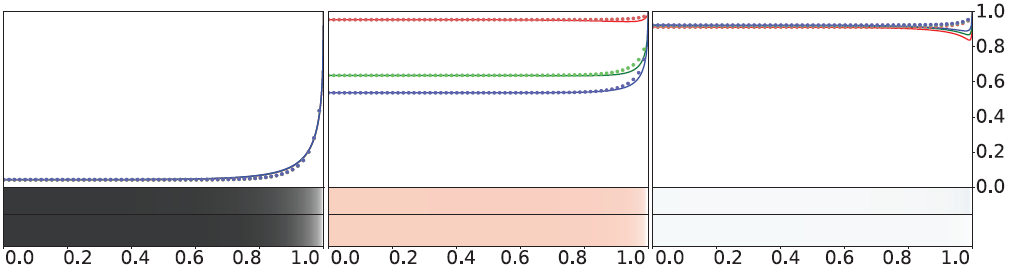
\includegraphics[width=12cm]{SchlickApproximation}
	\caption{From left to right the materials are, glass, copper and aluminium. Along the x-axis is plotted \begin{math}\sin(\theta_i)\end{math}, and along the y-axis is the intensities of each RGB channel. The solid lines are the actual Fresnel reflectance, and the dotted lines are the values given by the Schlick approximation. Similarly, the upper colour strip is the actual Fresnel reflectance, and the lower is that yielded from the Schlick approximation. Taken from~\cite{RTR4}.}
	\label{fig:SchlickApproximation}
\end{figure}

\subsubsection{NDF Implementations}

In this section we will only concern ourselves with \textit{isotropic} NDFs, which are those that are invariant when rotated about \begin{math}n\end{math}. \textit{Anisotropic} NDFs do exist and are crucial when rendering surfaces like brushed metal. A prominent isotropic NDF is the Beckmann distribution~\cite{Beckmann}. It is widely used in the field of optics and is the NDF of choice in the Cook-Torrance BRDF~\cite{WalterRefraction}~\cite{CookTorrance}. Walter et al give an equation for the Beckmann distribution~\cite{WalterRefraction}. After using some identities to manipulate it, the trigonometric functions can be replaced with dot products to yield the following:

\begin{equation}
	D(\vect{m}) = \frac{\mathcal{X}^+(\vect{m}\cdot\vect{n})}{\pi\alpha_b^2(\vect{m}\cdot\vect{n})^4}\exp(\frac{(\vect{m}\cdot\vect{n})^2 - 1}{\alpha_b^2(\vect{m}\cdot\vect{n})^2})
\end{equation}

\begin{math}\alpha_b\end{math} controls the roughness of the surface and thus the spread of the specular response~\cite{CookTorrance}.

The other NDF that has seen extensive use in the graphics community is the GGX distribution. Originally formulated by Trowbridge and Reitz in 1975, the GGX distribution only started to see use after it was reformulated by Walter et al in 2007~\cite{TrowbridgeAndReitz}\cite{WalterRefraction}. It has the following form:

\begin{equation} \label{eq:GGX}
	D(\vect{m}) = \frac{\alpha_g^2\mathcal{X}^+(\vect{m}\cdot\vect{n})}{\pi(1 + (\vect{m}\cdot\vect{n})^2(\alpha_g^2 - 1))^2}
\end{equation}

\begin{math}\alpha_g\end{math} is similarly used to control the roughness of the surface, although it scales in a different manner. Burley proposes mapping \begin{math}\alpha_g = r^2\end{math} where \begin{math}r\end{math} provides a perceptually linear change in roughness as it moves between 0 and 1~\cite{Burley2012Physically}. Exposing parameters to artists in this linear manner is a common trope in graphics. Karis outlines it as one of the key goals they pursued when migrating the Unreal Engine over to a PBR pipeline~\cite{RealShadingInUnreal}.

\subsubsection{Masking-shadowing Function Implementations}

Implementations of the masking-shadowing function depend on the NDF used. There are two main options to choose from. The first is a function created by Torrance and Sparrow, which considers adjacent microfacets to form a "V-groove cavity"~\cite{TorranceSparrowVCavity}. The second option is the Smith masking-shadowing function~\cite{SmithMaskingShadowingFunction}. Heitz thoroughly analyses the two models and concludes that whilst they are both physically based, the Smith function is more accurate to real materials, with the Torrence-Sparrow function producing too small a specular component for rough materials viewed at glancing angles~\cite{HeitzMicrofacetTheory}. The most accurate version of the Smith function is the \textit{Smith height-correlated masking-shadowing function}. This takes into account the height of surface points relative to the rest of the surface. This is significant because points that are lower in the surface are more likely to experience masking and shadowing~\cite{RTR4}.

The Smith height-correlated masking-shadowing function that is intended for use with the GGX NDF is~\cite{RTR4}:

\begin{equation} \label{eq:SmithGGXFunction}
	G(\vect{l}, \vect{v}, \vect{m}) = \frac{\mathcal{X}^+(\vect{m}\cdot\vect{v})\mathcal{X}^+(\vect{m}\cdot\vect{l})}{1 + \Lambda(a_{\vect{v}}) + \Lambda(a_{\vect{l}})}
\end{equation}

where

\begin{equation}
	\Lambda(a) = \frac{-1 + \sqrt{1 + \frac{1}{a^2}}}{2}
\end{equation}

and

\begin{gather*}
	a_{\vect{v}} = \frac{\vect{n}\cdot\vect{v}}{\alpha_g\sqrt{1 - (\vect{n}\cdot\vect{v})^2}}
	\quad
	a_{\vect{l}} = \frac{\vect{n}\cdot\vect{l}}{\alpha_g\sqrt{1 - (\vect{n}\cdot\vect{l})^2}}
\end{gather*}

\subsection{Diffuse BRDFs} \label{DiffuseBRDFs}

We now focus on diffuse BRDFs, which model the local subsurface scattering component of local reflectance. Similar to the intrinsic specular colour of a material, \begin{math}F_0\end{math}, we also define an intrinsic diffuse colour called the \textit{subsurface albedo}. Denoted by \begin{math}\rho_{ss}\end{math}, this is the proportion of transmitted light that is re-emitted at the surface via subsurface scattering. Since this amount is a distribution of wavelengths, \begin{math}\rho_{ss}\end{math} is represented as an RGB triplet. The more \begin{math}\rho_{ss}\end{math} tends towards \begin{math}(0, 0, 0)\end{math}, the more absorption takes place within the interior of the associated material.

Diffuse BRDFs can be placed into two categories: those that are built upon microfacet theory and account for surface roughness; and those that don't utilise microfacet theory and just assume the surface is flat. As explained by Akenine-M\"{o}ller et al, the type of model to use is determined by the differences between the size of the microgeometry, and the subsurface scattering distances~\cite{RTR4}. If the microgeometry is larger than the scattering distances, then a rough-surface diffuse BRDF should be used. If the microgeometry is smaller than the scattering distances, then a flat-surface diffuse BRDF can be used.

\subsubsection{Flat-surface Diffuse BRDFs}

The most common diffuse BRDF is based on Lambertian reflection and has the following formulation:

\begin{equation} \label{eq:LambertianDiffuse}
	f_{diff}(\vect{l}, \vect{v}) = (1 - F(\vect{h}, \vect{l}))\frac{\rho_{ss}}{\pi}
\end{equation}

The \begin{math}\pi\end{math} is obtained by setting the \textit{directional-hemispherical reflectance function} to a constant value and integrating it over all values of \begin{math}\vect{v}\end{math}~\cite{RTR4}. The inclusion of the Fresnel reflectance ensures that only light that was transmitted into the interior of the object is available to the diffuse term~\cite{ShirleySimpleConservationOfEnergy}. This helps to comply with the law of conservation of energy. When the \begin{math}(1 - F(\vect{h}, \vect{l}))\end{math} is removed from equation \ref{eq:LambertianDiffuse}, what is left is commonly referred to as the Lambertian BRDF.

Equation \ref{eq:LambertianDiffuse} has a constant value for all view directions. The physical basis for such a formulation is rooted in the observation that, prior to re-emission, subsurface scattered light will undergo many scattering events in the interior of the object (as explained in section \ref{PhysicsOfLightMatterInteraction}). This has the effect of randomising the directions of outgoing light, which can be intuitively modelled as a constant value over all \begin{math}\vect{v}\end{math}~\cite{HammonBRDF}. However, real materials will show some directional bias, whether that's due to refraction or the need to respect Helmholtz reciprocity (which equation \ref{eq:LambertianDiffuse} violates)~\cite{RTR4}. Shirley et al present a more accurate diffuse BRDF that is partially coupled with the specular component~\cite{PractitionersReflectionModels}.

\subsubsection{Rough-surface Diffuse BRDFs}

The most notable microfacet-based, rough-surface diffuse BRDF is that created by Oren and Nayar~\cite{OrenAndNayar}. It is comprised of: a gaussian NDF; a Torrence-Sparrow masking-shadowing function; and a constant micro-BRDF that models each microfacet as a perfectly diffuse surface. The Oren-Nayar BRDF increases in intensity as \begin{math}\vect{v}\end{math} approaches \begin{math}\vect{l}\end{math}, a property that is coherent with the reflectance characteristics of rough surfaces like clay~\cite{OrenAndNayar}. As a result, their BRDF produces much more realistic results for these rough surfaces when compared to the Lambertian BRDF. Alternative diffuse BRDFs that are based on microfacet theory are given by Gotanda, and another by Hammon~\cite{GotandaDiffuseBRDF}\cite{HammonBRDF}. These both make use of the more modern GGX distribution and Smith height-correlated masking-shadowing function.

Burley presents a BRDF that accounts for roughness, but does not use microfacet theory~\cite{Burley2012Physically}. Instead, it is empirically constructed by observing how light responds to different materials in the \textit{MERL} BRDF database. The Frostbite Engine utilises a slightly modified version of Burley's BRDF, where it has been tweaked to respect energy conservation~\cite{MovingFrostbitetoPBR}.

\subsection{Illumination} \label{Illumination}

Having thoroughly examined the BRDF, we now study the other function in the reflectance equation, the incoming radiance, \begin{math}L_i(\vect{p}, \vect{l})\end{math}.

In section \ref{BlinnPhongShading}, a distinction was made between direct and indirect illumination. Direct illumination is light that arrives directly from a light source. Indirect illumination is light that only strikes point \begin{math}\vect{p}\end{math} after first undergoing collisions with other objects and media within the scene. When considering the unit hemisphere of incoming light, direct illumination contributes high levels of radiance, over small solid angles. Indirect illumination then spans the rest of the hemisphere, with small to moderate levels of radiance. This difference means that when integrating the reflectance equation over all possible incident light directions, it is common to deal with direct and indirect light sources separately.

\subsubsection{Indirect Illumination}

Indirect illumination impinging upon \begin{math}\vect{p}\end{math} can be computed using \textit{Global Illumination} (GI) or \textit{Local Illumination} techniques. GI algorithms determine \begin{math}L_i(\vect{p}, \vect{l})\end{math} by backtracking, and explicitly simulating the previous light-matter interactions that have led to that illumination. Such techniques are dependent on having a global view of the objects in the scene at each shading point. The ray tracing algorithm briefly discussed in the Introduction is a GI technique. The tremendous amount of realism and detail that GI techniques yield, unfortunately demand an equally tremendous amount of compute time. The frame times given for ray tracing was indicative of this. As a result, GI algorithms cannot be computed per frame in real-time rendering. However, for static environments, GI can be used to precompute some aspects of lighting, which are then retrieved at run time. This process is known as \textit{baking}~\cite{UberBake}.

Local Illumination techniques do not require a global view of scene objects; they only need to be aware of the current object that is being shaded. We have already examined a crude Local Illumination technique for modelling indirect illumination: the ambient term presented in section \ref{BlinnPhongShading}. More advanced techniques are Image Based Lighting and Irradiance Mapping~\cite{HoffmanPBSBackground}\cite{IrradianceMaps}.

\subsubsection{Direct illumination}

Computing the direct illumination incident to \begin{math}\vect{p}\end{math} involves integrating the reflectance equation over specific, known values of \begin{math}\vect{l}\end{math}. There are three types of light sources: area, punctual and directional. Area lights, as the name suggests, have a size, as well as a location. When projected onto the unit hemisphere, this size translates to a solid angle. Therefore, to work out the contribution of incoming radiance from that area light, an integration is done over values of \begin{math}\vect{l}\end{math} that lie within its projected solid angle.

Punctual lights are similar to area lights, except they have an infinitesimally small size. This simplifies the evaluation of the reflectance equation because only one direction \begin{math}\vect{l}\end{math} needs to be integrated for each punctual light source. However, punctual lights are an abstraction of the real world - all lights occupy some area - and therefore the simplified computation they provide comes at a cost. Point lights will produce very small specular highlights on shiny materials, which looks unrealistic. To combat this, artists will often increase the roughness of the material to spread the highlight out, but in doing so they couple the specific lighting environment and material properties together~\cite{MovingFrostbitetoPBR}~\cite{RealShadingInUnreal}. In the Introduction we discussed why such a practise can be problematic.

Directional lights are then a further simplification, where they are assumed to be positioned so far away, that their direction is constant over all objects in the scene. Thus, they are not associated with a particular location.

\subsubsection{Point Lights}

The most common form of punctual light is the point light. A point light emits constant radiance over all directions. The colour of the point light is denoted as \begin{math}\vect{c}_{PL}\end{math}, which is an unbounded RGB triplet~\cite{HoffmanPBSBackground}. \begin{math}\vect{c}_{PL}\end{math} is then defined as the reflected radiance from a perfectly diffuse white surface that directly faces the light. Given this definition, Hoffman derives a simplified version of the reflectance equation for a single point light~\cite{HoffmanPBSBackground}. Extending this for multiple point lights, the reflectance equation becomes:

\begin{equation} \label{eq:PointLightsReflectanceEquation}
	L_o(\vect{p}, \vect{v}) = \pi\sum_{i = 0}^{N - 1}f(\vect{l}_{PL_i}, \vect{v})\vect{c}_{PL_i}(\vect{n}\cdot\vect{l}_{PL_i})^+
\end{equation}

where \begin{math}N\end{math} is the number of point lights.

Light intensity is attenuated as the distance between the light source and shaded point \begin{math}\vect{p}\end{math} increases. For point lights, this attenuation is equal to the inverse of the squared distance. Therefore, \begin{math}\vect{c}_{PL_i}\end{math} will be proportional to \begin{math}1 / distance^2\end{math}. The dot product term has been clamped to 0, so that the contribution of point lights that are located below the surface is discarded.

\subsection{Dynamic Range and Displays} \label{DynamicRangeAndDisplays}

When rendering, a distinction can be made between the \textit{dynamic range} of values produced via shading, and the dynamic range supported by the display. Dynamic range is defined as the ratio between the highest and lowest brightness values. Most displays are only capable of \textit{Low Dynamic Range} (LDR), which means the maximum value of RGB triplets that they can display is restricted to 1 for each channel. However, real world brightness values, which shading seeks to emulate, often span a much greater range~\cite{Reinhard}. This range is called \textit{High Dynamic Range} (HDR). RGB triplets that measure HDR values have practically no restriction on the upper values for their components. It is therefore necessary to provide a mechanism that converts between HDR RGB triplets and LDR RGB triplets. This conversion process is called \textit{tone mapping}~\cite{HoffmanKeynoteEchoChamber}. A good \textit{tone mapping operator} seeks to recreate on the display, the perceptual impression that a viewer would experience if they were present in the real life scene~\cite{HoffmanKeynoteEchoChamber}. This is known as \textit{image reproduction}.

\subsubsection{Tone Mapping}

In a non-physically based renderer, where the Blinn-Phong shading model might be employed, the discrepancy is dealt with by simply performing all shading calculations in LDR, and passing the values directly to the display. This behaviour is essentially equivalent to employing a tone mapping operator that clamps all RGB values to 1 per channel. As explained above, the dynamic range of the real world far outstrips LDR, so this necessarily hampers the shading ability of non-physically based renderers. Either they artificially compress the brightness range in the scene, or all the bright pixel values just become white, with the detail between them being lost. Neither approach is desirable.

A physically based renderer is focused on simulating real world light-matter interaction, so Physically Based Shading is done in the HDR space of RGB triplets. This is why the \begin{math}\vect{c}_{PL}\end{math} RGB triplet presented in section \ref{Illumination} was unbounded. This ensures that the vast brightness differences that exist between elements in a scene - for example, the vast difference that will exist between the radiance of the sun and that of a weak point light - can be accurately represented when shading. Once shaded, the HDR RGB triplet is tone mapped to obtain the LDR value that is submitted to the display. Crucially, this tone mapping is done in a more advanced way than the clipping above, with image reproduction being the goal. All tone mapping operators that have this aim are based around the \textit{sigmoid function}~\cite{HoffmanKeynoteEchoChamber}. This function provides a smooth roll off of values, so that some of the detail in the darkest and brightest elements of the frame is preserved.

One of the early tone mapping operators used in real-time rendering is given by Reinhard et al~\cite{Reinhard}. More recently, the use of \textit{filmic} operators, that emulate the image reproduction properties of photographic film, has been widely adopted. This was spearheaded by Hable, who created an operator that was first used in the game Uncharted 2~\cite{Hable}. Building on this concept, the \textit{Academy Colour Encoding System} (ACES) is a standard that prescribes how colour should be managed in movies and TV. It has since spread into real-time rendering, being the tone mapping operator of choice in the Unreal Engine~\cite{ACESUnreal}.

\subsubsection{Exposure}

A closely related topic to tone mapping is \textit{exposure}. Exposure is used to scale HDR RGB triplets before they are tone mapped; it has the effect of altering the overall brightness level of a rendered frame. Exposure can be set statically per scene, or computed dynamically by statistically analysing the brightness levels of previous frames~\cite{RTR4}.

\subsubsection{Gamma Correction}

Humans do not perceive radiance in a linear manner, with absolute differences in lower values being much more noticeable than the same differences in higher values. This means that if a human is given a uniform range of radiance values, they will perceive it as entirely non-uniform in its brightness - colours will be seen to rise very quickly towards white. Displays compensate for this perceptual phenomena by mapping input radiance values to non-linear output values. For most displays, this mapping is done in accordance with the \textit{sRGB display transfer function}. In this way, a display outputs colours that are perceived as uniform by humans. However, when rendering, we want the display to output the exact radiance values we give to it, since these have been accurately calculated via shading. Therefore, as the final step before colours are submitted to the display (after tone mapping and exposure have been applied), we apply the inverse of the sRGB display transfer function to all radiance values. This is known as \textit{gamma correction}. Gritz and d'Eon detail the artifacts that can occur if gamma correction is not performed~\cite{GPUGemsChapter24}. Gamma correction can be approximated by raising all radiance values to the power of \begin{math}2.2\end{math}, or done more accurately by using the exact inverse of the sRGB display transfer function~\cite{MovingFrostbitetoPBR}.